\documentclass{article}
\usepackage[magyar]{babel}
\usepackage{t1enc}
\usepackage{lipsum}
\usepackage{hulipsum}
\usepackage{tikz}
\usetikzlibrary{patterns}
\usetikzlibrary{shapes} 


\begin{document}

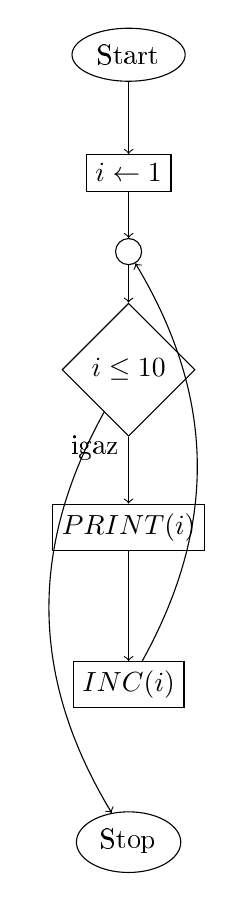
\begin{tikzpicture}
\path (0,0) node[ellipse,draw](Start) {Start}
(0,-1.5) node[rectangle,draw](i_1) {$i \leftarrow 1$}
(0,-2.5) node[circle,draw](c) {}
(0, -4) node[diamond,draw](i_10) {$i \leq 10$}
(0, -6) node[rectangle,draw](i_print) {$PRINT(i)$}
(0, -8) node[rectangle,draw](i_inc) {$INC(i)$}
(0,-10) node[ellipse,draw](Stop) {Stop}
;
\draw[->] (Start) -- (i_1);
\draw[->] (i_1) -- (c);
\draw[->] (c) -- (i_10);
\draw[->] (i_10) -- (i_print);
\draw (i_10) -- (0,-5) node[left] {igaz};
\draw[->] (i_print) -- (i_inc);

\draw (i_inc) edge[->,bend right] (c);
\draw (i_10) edge[->,bend right] (Stop);

\end{tikzpicture}

\end{document}